% One KDense layer as two batched matrix products. Compile standalone.
\documentclass[tikz,border=4pt]{standalone}
\usepackage{amsmath,amssymb}
\usepackage{mathptmx}
\usepackage[scaled=0.90]{helvet}
\usetikzlibrary{arrows.meta,positioning,calc,fit,backgrounds}

\definecolor{ink}{RGB}{28,32,38}
\definecolor{primary}{RGB}{155,26,32}
\definecolor{accentsoft}{RGB}{247,228,229}
\definecolor{rule}{RGB}{209,213,219}
\definecolor{panel}{RGB}{250,250,251}
\definecolor{blueacc}{RGB}{30,90,168}
\definecolor{bluesoft}{RGB}{232,239,248}
\definecolor{muted}{RGB}{95,107,122}

\begin{document}
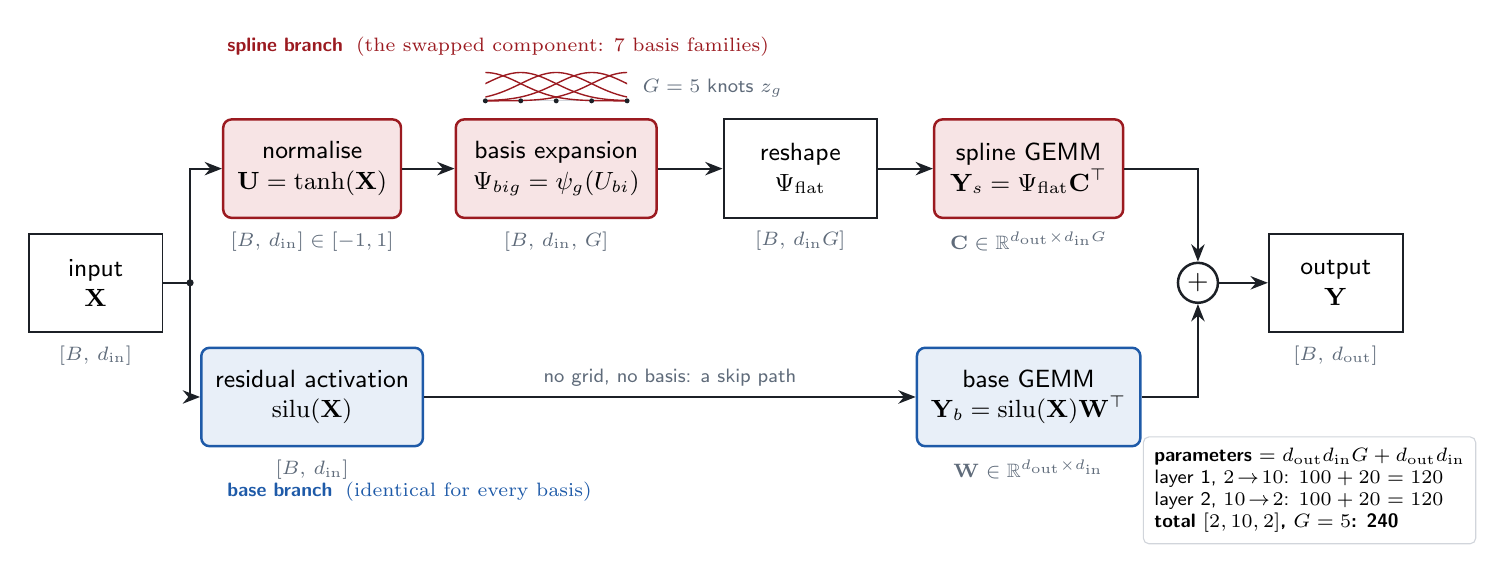
\begin{tikzpicture}[
  font=\sffamily\small, >={Stealth[length=2.2mm,width=1.7mm]},
  tensor/.style={draw=ink, fill=white, line width=0.7pt, align=center, inner sep=5pt, minimum height=1.25cm},
  spl/.style={draw=primary, fill=accentsoft, rounded corners=3pt, line width=0.9pt, align=center, inner sep=5pt, minimum height=1.25cm},
  bas/.style={draw=blueacc, fill=bluesoft, rounded corners=3pt, line width=0.9pt, align=center, inner sep=5pt, minimum height=1.25cm},
  flow/.style={->, line width=0.8pt, draw=ink},
  dims/.style={font=\sffamily\scriptsize\color{muted}},
  lane/.style={font=\sffamily\scriptsize\bfseries},
]
\def\yt{1.45}
\def\yb{-1.45}
% ---------------------------------------------------------------- nodes
\node[tensor, minimum width=1.7cm] (x) at (0,0) {input\\$\mathbf{X}$};
\node[dims, below=1pt of x] {$[B,\,d_{\mathrm{in}}]$};

\node[spl, minimum width=2.0cm] (norm) at (2.75,\yt) {normalise\\$\mathbf{U}=\tanh(\mathbf{X})$};
\node[dims, below=1pt of norm] {$[B,\,d_{\mathrm{in}}]\in[-1,1]$};

\node[spl, minimum width=2.55cm] (psi) at (5.85,\yt) {basis expansion\\$\Psi_{big}=\psi_g(U_{bi})$};
\node[dims, below=1pt of psi] {$[B,\,d_{\mathrm{in}},\,G]$};
% tiny glyph of the G=5 grid above the expansion
\begin{scope}[shift={($(psi.north)+(-0.9,0.22)$)}, x=0.36cm, y=0.36cm]
  \draw[rule] (0,0) -- (5,0);
  \begin{scope}
    \clip (0,-0.05) rectangle (5,1.1);
    \foreach \z in {0,1.25,2.5,3.75,5}
      \draw[primary, line width=0.5pt, domain=-1.5:6.5, samples=60, smooth]
        plot (\x, {exp(-0.5*((\x-\z)/1.25)^2)});
  \end{scope}
  \foreach \z in {0,1.25,2.5,3.75,5} \fill[ink] (\z,0) circle (0.9pt);
  \node[dims, anchor=west] at (5.2,0.45) {$G=5$ knots $z_g$};
\end{scope}

\node[tensor, minimum width=1.95cm] (flat) at (8.95,\yt) {reshape\\$\Psi_{\mathrm{flat}}$};
\node[dims, below=1pt of flat] {$[B,\,d_{\mathrm{in}}G]$};

\node[spl, minimum width=2.4cm] (C) at (11.85,\yt) {spline GEMM\\$\mathbf{Y}_s=\Psi_{\mathrm{flat}}\mathbf{C}^{\top}$};
\node[dims, below=1pt of C] {$\mathbf{C}\in\mathbb{R}^{d_{\mathrm{out}}\times d_{\mathrm{in}}G}$};

\node[bas, minimum width=2.0cm] (silu) at (2.75,\yb) {residual activation\\$\mathrm{silu}(\mathbf{X})$};
\node[dims, below=1pt of silu] {$[B,\,d_{\mathrm{in}}]$};

\node[bas, minimum width=2.4cm] (W) at (11.85,\yb) {base GEMM\\$\mathbf{Y}_b=\mathrm{silu}(\mathbf{X})\mathbf{W}^{\top}$};
\node[dims, below=1pt of W] {$\mathbf{W}\in\mathbb{R}^{d_{\mathrm{out}}\times d_{\mathrm{in}}}$};

\node[circle, draw=ink, fill=white, line width=0.9pt, inner sep=1.5pt, font=\normalsize] (sum) at (14.0,0) {$+$};
\node[tensor, minimum width=1.7cm] (y) at (15.75,0) {output\\$\mathbf{Y}$};
\node[dims, below=1pt of y] {$[B,\,d_{\mathrm{out}}]$};

% ---------------------------------------------------------------- edges
\draw[line width=0.8pt, draw=ink] (x.east) -- (1.2,0);
\fill[ink] (1.2,0) circle (1.3pt);
\draw[flow] (1.2,0) |- (norm.west);
\draw[flow] (1.2,0) |- (silu.west);
\draw[flow] (norm) -- (psi);
\draw[flow] (psi) -- (flat);
\draw[flow] (flat) -- (C);
\draw[flow] (silu) -- node[above, dims] {no grid, no basis: a skip path} (W);
\draw[flow] (C.east) -| (sum.north);
\draw[flow] (W.east) -| (sum.south);
\draw[flow] (sum) -- (y);

% ---------------------------------------------------------------- lane labels
\node[lane, text=primary, anchor=west] at (1.55,3.0) {spline branch \;{\normalfont\scriptsize(the swapped component: 7 basis families)}};
\node[lane, text=blueacc, anchor=west] at (1.55,-2.65) {base branch \;{\normalfont\scriptsize(identical for every basis)}};

% parameter count for the Lotka--Volterra network
\node[draw=rule, fill=white, rounded corners=2pt, align=left, font=\sffamily\scriptsize, inner sep=4pt, anchor=north west]
  at (13.3,-1.95)
  {\textbf{parameters} $=d_{\mathrm{out}}d_{\mathrm{in}}G+d_{\mathrm{out}}d_{\mathrm{in}}$\\
   layer 1, $2\!\to\!10$: $100+20=120$\\
   layer 2, $10\!\to\!2$: $100+20=120$\\
   \textbf{total $[2,10,2]$, $G=5$: 240}};
\end{tikzpicture}
\end{document}
